\documentclass[../main.tex]{subfiles}
\graphicspath{{\subfix{../images/}}}
\begin{document}


\section{Arc length}
The length of an arc along a portion of a curve, like volumes of revolution, can be found by definite integration.

To derive the formula for the arc length, we need to be aware of the Mean Value Theorem. This states that if a function is continuous over a closed interval $[a, b]$ then there exists a point somewhere within that range that has a gradient equal to the functions' average rate of change over the range.

You can see that this must logically be the case by looking at the diagram below. You can clearly see that there must be a point somewhere in the interval $[a,b]$ where the tangent will have the same gradient as the straight line from point $a$ to point $b$.

\begin{figure}[h]
    \centering
    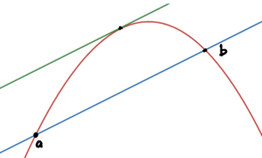
\includegraphics[width=0.3\linewidth]{images/arclength1.png}
\end{figure}

To approximate the length of the arc over an interval $[a,b]$, we first divide the interval into $n$ equal sub-intervals, each of width $\Delta x$. We denote each point on the curve $P_i$, and we can approximate the curve by creating straight lines between each point. Below is an example with 13 points.

\begin{figure}[h]
    \centering
    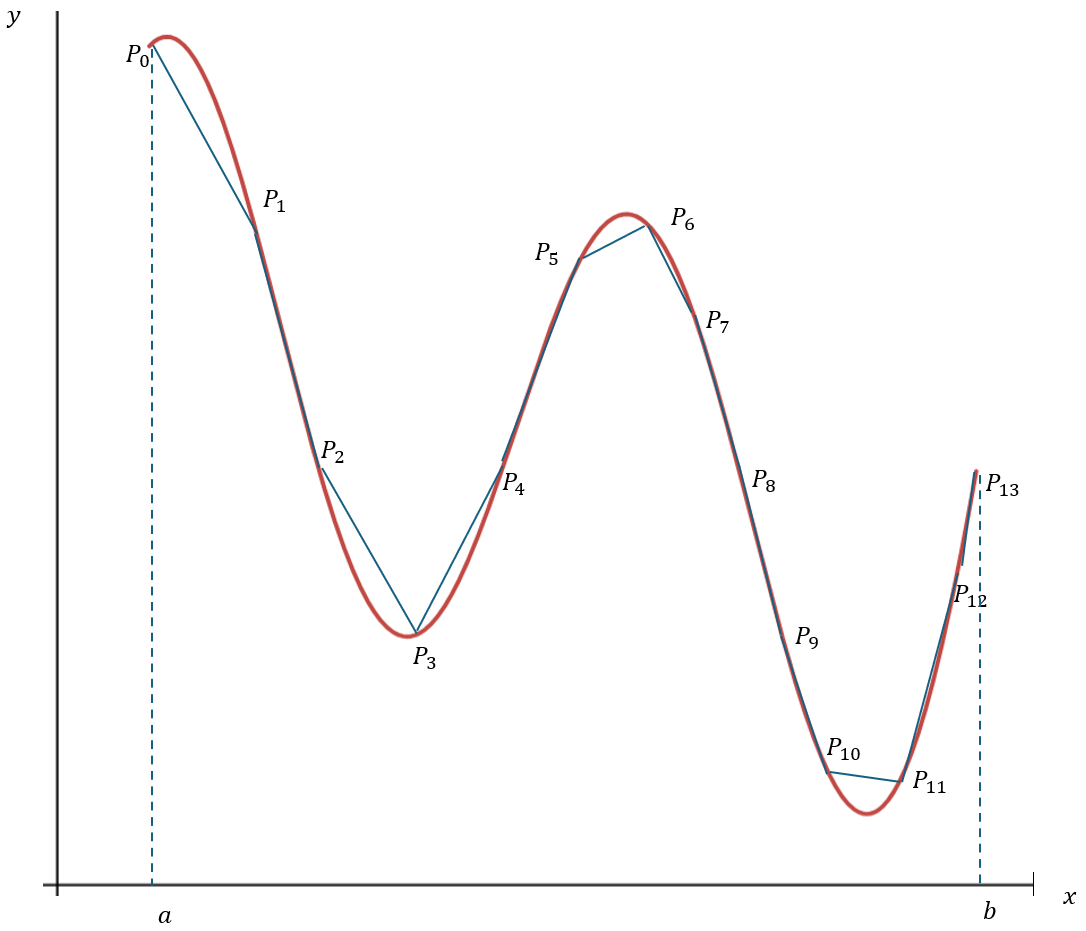
\includegraphics[width=0.6\linewidth]{images/arclength5.png}
\end{figure}

If we write each of those line segments as $|P_{i-1} P_{i}|$, the length of the curve will be approximately $L\approx \sum\limits_{i=1}^n |P_{i-1} P_i|$.

We can get the exact length by making $n$ larger and larger, giving:

\[L=\lim\limits_{n \Rightarrow \infty} \sum\limits_{i=1}^n |P_{i-1} P_i|\]


The length of each of these line segments could be found by using Pythagoras' Theorem. 

If the change in $x$ is constant ($\Delta x$), and the change in the height of the function is $\Delta y_n$, as below:

\begin{figure}[h]
    \centering
    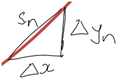
\includegraphics[width=0.2\linewidth]{images/arclength3.png}
\end{figure}

We can calculate the length of the $n^{th}$ line segment with:

\[s_n=\sqrt{(\Delta x)^2+(\Delta y_n)^2}\]


This is where the Mean Value Theorem comes in. By this theorem, there exists a point $x_n$ with a length of $\Delta x$ such that $\Delta y_n=f'(x_n)\times \Delta x$. This comes from the fact that gradient is rise over run, so the gradient at point $x_n$ (which can be expressed as $f'(x_n)$) will be $\frac{\Delta y_n}{\Delta x}$.

\textit{(In other words, the change in y is equal to the gradient multiplied by the change in x)}

This means we can rewrite the line segment length as $s_n=\sqrt{(\Delta x)^2+(f'(x_n)\times \Delta x)^2}$

Which can be simplified as $s_n=\sqrt{1+(f'(x_n))^2}\Delta x$.

\textbf{Note:} The function and its derivative \textbf{must be continuous} on the closed interval being considered for the arc length calculation to be guaranteed of accuracy.

The arc length is now just a sum of an infinite number of infinitely small lengths:

\[L=\lim\limits_{n \Rightarrow \infty} \sum\limits_{i=1}^n \sqrt{1+(f'(x_n))^2} \Delta x\]

By the definition of the definite integral, this just means the length is:

\[L=\int_a^b \sqrt{1+(f'(x))^2}\,dx\]

\pagebreak
\subsection*{Example}
Find the length of the arc on the function $f(x)=\frac{1}{3}x^{\frac{3}{2}}$ on the interval $[0,5]$.

\begin{figure}[h]
    \centering
    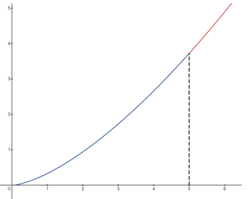
\includegraphics[width=0.3\linewidth]{images/arclength4.png}
\end{figure}

$f(x)=\frac{1}{3}x^{\frac{3}{2}}$

$f'(x)=\frac{1}{2}x^{\frac{1}{2}}$

Because both of these are continuous on the interval from $x=0$ to $x=5$, we can use the arc length formula.

$L=\int_0^5 \sqrt{1+\Bigl(\frac{1}{2}x^{\frac{1}{2}}\Bigr)^2}\,dx$

$L=\int_0^5 \sqrt{1+\frac{x}{4}}\,dx$

$L=\Bigl[\frac{8}{3}(1+\frac{x}{4})^{\frac{3}{2}}\Bigr]_0^5$

$L=\frac{19}{3}$

\pagebreak
\hypertarget{arclengthlink}{\subsection*{Questions}}
\hyperlink{arclengthanswers}{(Answers - page {\pageref*{Arc length answers}})}

\label{Arc length}
\begin{enumerate}[itemsep=0.7cm]
    \item 
    Determine the length of the arc along the function $y=7(6+x)^{\frac{3}{2}}$ along the interval $[3,19]$

    \item
    Determine the length of the arc along the function $y=1+6x^{\frac{3}{2}}$ along the interval $[0,1]$

    \item 
    Determine the length of the arc along the function $y=\frac{3}{2}x^{\frac{2}{3}}$ along the interval $[1,8]$

    \item 
    Determine the length of the arc along the function $x=\frac{1}{3}(y^2+2)^{\frac{3}{2}}$ along the interval $0\leq y \leq 4$

    \item 
    Determine the length of the arc along the function $x=\frac{1}{3}\sqrt{y}(y-3)$ along the interval $1\leq y \leq 9$

    \item 
    Find the length of the arc for $y=\ln{(\cos{x})}$ on the closed interval $0 \leq x \leq \frac{\pi}{3}$

\end{enumerate}





\end{document}